% include the figures path relative to the master file
\graphicspath{{./content/intro/figures/}}

\section{Polarized cues used for attitude estimation}
\label{sec:pcues}

% solar zenith: angle between the zenith and the center of the sun disk $\theta_s$
% solar elevation: altitude of the sun, angle between the horizon and the
% center of the sun disk $\alpha_s$
% solar azimuth: direction of the sun $\phi_s$, while $\theta_s, \alpha_s$
% define how high is the sun
% scattering angle $\lambda$: angular distance between the observed celestial
% point and the sun
% solar meridian: plane containing the sun and the observer
% Scattering plane: plane of observer,  celestial point observed and the sun
% Rayleigh model- direction of polarization is perpendicular to the scattering
% plane

\subsection{Rayleigh scattering model}
\label{subsec:rayleigh}
The unpolarized sunlight passing through our atmosphere gets scattered by
different particles within the atmosphere.  Beside deviating the direction of
propagate wave, this transition also changes the polarization state of the
incident light. This transition can be explained using Rayleigh scattering
model.  Rayleigh scattering describes the scattering of light or any
electromagnetic waves by particles much smaller than their transmission
wavelength. Accordingly it assumes that scattering particles of the atmosphere
are small, homogeneous particles much smaller than the wavelength of the
sunlight.  Despite its simplification and assumption, this model proved to be
sufficient for describing skylight scattering and polarization
patterns~\cite{pomozi2001clearsky, horvath2002ground}.

The Rayleigh scattering model predicts that the unpolarized sunlight becomes
linearly polarized passing through the atmosphere. The polarization state of
the light or any electromagnetic wave can be expressed in terms
stokes parameters~\cite{goldstein2017polarized}.  Equation
\ref{eq:1} shows the stokes parameters for natural light after and before
passing through the atmosphere, since the last stokes parameter is $0$ after
scattering, the light is considered to be linearly polarized.
\begin{equation}
  \label{eq:1}
  s_{unp} =
  \begin{bmatrix}
    1\\0\\0\\0
  \end{bmatrix}
  \xrightarrow[]{\text{scattering}}
  s_{p}=
  \begin{bmatrix}
   s_0 \\ s_1 \\ s_2 \\ 0
 \end{bmatrix}
\end{equation}

Having polarization state of light, the \gls{dopl} ($\rho_{l}$) in terms of stokes
parameters and the scattering angle ($\gamma$), respectively is presented as:
\begin{equation}
  \label{eq:2}
  \rho_{l} = \frac{\sqrt{s_{1}^{2}+s_{2}^{2}}}{s_0} =
  \frac{\sin^{2}(\gamma)}{\cos^{
      2}(\gamma)+1}
\end{equation}
\noindent where scattering angle $\gamma$ is the angular distance between the
celestial point observed and the sun.
According to Rayleigh model, the \gls{dopl}, $\rho_{l}$, varies
from 0 to $\approx 1$ depending on the scattering angle, $\gamma$, ($\rho_{l} =
0$ while $\gamma = 0, \pi$ and $\rho_{l} \approx 1$ while $\gamma =
\pi/2$)~\cite{smith2007polarization, miyazaki09sunlightpolarization}.
Accounting for the approximation and polarization defect, Eq.~\ref{eq:2}
is presented as~\cite{pomozi2001clearsky}:
\begin{equation}
  \label{eq:3}
  \rho_{l} = \rho_{l_{max}}\frac{1 - \cos^{2}(\gamma)}{1 + \cos^{
      2}(\gamma)}
\end{equation}


\subsection{Polarization by scattering model for sky pattern}
\label{subsec:pscattering}
This section represent the relations between polarized measurements in pixel
frame $\mathcal{P}$ and sun and celestial point in the world frame
$\mathcal{W}$.

Based on Rayleigh scattering the electric field of incident light after
scattering is perpendicular to the scattering plane, that is defined by the
observer, celestial point and the sun.
This plane is highlighted by light shade of red in Fig.~ref{fig:scattering} and
is represented by a sun vector $\vec{s}$ and celestial vector $\vec{c}$.

\begin{figure}
  \centering
  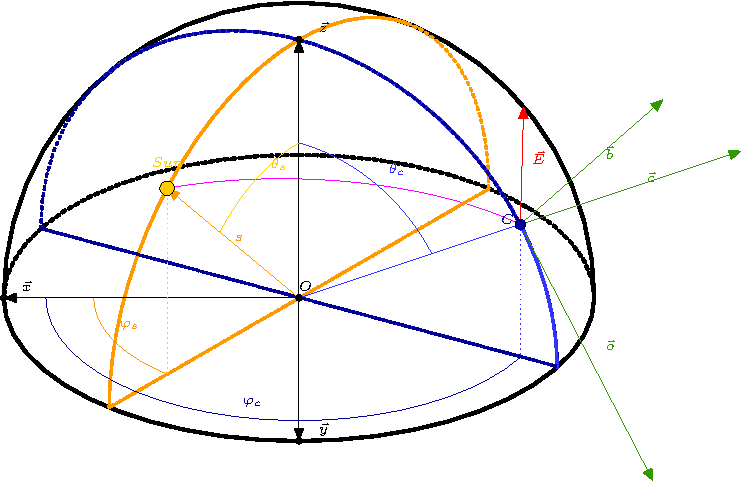
\includegraphics[width=0.5\textwidth]{./content/intro/figures/polasky4-crop.pdf}
  \label{fig:scattering}
  \caption{Skylight polarization by scattering\textcolor{red}{The figure needs
      to be re-designed according the text}}
\end{figure}
Accordingly the normalized electric field vector $\vec{E}$ in the world frame
is presented as the normalized cross product of $\vec{s}$ and
$\vec{c}$ (see Eq.~\ref{Eq:E}).

\begin{equation}
\vec{E}=\frac{\vec{s}\wedge \vec{c}}{\left\Vert \vec{s}\wedge
    \vec{c}\right\Vert }
\label{Eq:E}
\end{equation}

However measuring the skylight polarization pattern and \gls{aop}, the electric
field in the pixel frame $\mathcal{P}$ ($\widehat{obc}$) is represented as:
\begin{equation}
E_{obc}=\left[\begin{array}{l}
E_{o}\\
E_{b}\\
0
\end{array}\right]=\left[\begin{array}{l}
\cos\alpha\\
\sin\alpha\\
0
\end{array}\right]
\label{Eq:Eproj}
\end{equation}
\noindent where $\alpha$ is the measured \gls{aop}.
Combination of equation~(\ref{Eq:E}) and (\ref{Eq:Eproj}) and using the
scattering angle $\gamma$, between $\vec{s}$ and $\vec{c}$ leads to:
\begin{equation}
\begin{cases}
(s\wedge c)\cdot o & =\sin\gamma\cos\alpha\\
(s\wedge c)\cdot b & =\sin\gamma\sin\alpha
\end{cases},\label{eq:E0EB vect-1-1}
\end{equation}

\noindent applying vector triplet cross product rule on Eq.~\ref{eq:E0EB
  vect-1-1} results.
\begin{equation}
\begin{cases}
s\cdot b & =\sin\gamma\cos\alpha\\
s\cdot o & =-\sin\gamma\sin\alpha
\end{cases}\label{eq:scal-b-o}
\end{equation}

Considering the \gls{dopl} (see Eq.~\ref{Eq:3}), the scattering angle
$\gamma$, therefore can be represented as:
\begin{equation}
\cos\gamma=s\cdot c=\pm\sqrt{\frac{1-\rho_{l}'}{1+\rho_{l}'}}
\label{Eq:cosg}
\end{equation}
\noindent with $\rho_{l}'=\frac{\rho_{l}}{\rho_{l_{max}}}.$

Equations~\ref{eq:scal-b-o} and \ref{Eq:cosg} finally leads to the sun vector
in pixel frame $\mathcal{P}$ which express a direct relation between the
measured polarization parameters (\gls{aop} ($\alpha$), \gls{dopl} ($\rho$)),
scattering angle ($\gamma$), the sun position,  and the celestial point:
\begin{equation}
  \label{Eq:sunp}
  \vec{s}_{\mathcal{P}} =
  \left[
    \begin{array}{l}
    -\sin\gamma \sin\alpha\\
    \sin\gamma \cos\alpha\\
    \cos\gamma
  \end{array}
  \right]
\end{equation}

\subsection{Attitude estimation and polarization by scattering of skylight}
\label{subsec:ps-attitude}

% \begin{equation}
% R^{t}\cdot s=R_{cp}\left[\begin{array}{c}
% -\sin\gamma\sin\alpha\\
% \sin\gamma\cos\alpha\\
% \cos\gamma
% \end{array}\right]=v,\label{eq:qtrans}
% \end{equation}
% where $v$ is a vector obtained from polarization measurements according
% to the selected pixel.



% \begin{itemize}
% \item[] Scattering plane - is the plane defined by the observer, celestial point and
%   the sun.
% \item[] Meridional plane - is the plane defined by the local zenith and the
%   celestial point

% \item[] Solar meridional plane - is the plane defined by the sun and the observer
% \item[] Scattering angle $\lambda$ is the angular distance between celestial point
%   observed and the sun
% \end{itemize}

% Some stuff that emac's colegues use
%%% Local Variables:
%%% mode: late
%%% TeX-master: "../../main.tex"
%%% End: \section{Polarized cues used for attitude estimation}
